\begin{frame}[allowframebreaks]{Handling imbalanced data}
\begin{itemize}
    \item \textbf{Problem:}
    \begin{itemize}
        \item You have a majority class with many more examples than the minority class
        \item Or: classes are balanced, but associated costs are not (e.g., FN worse than FP)
    \end{itemize}

    \item \textbf{Solutions we’ve already covered:}
    \begin{itemize}
        \item Add class weights to the loss function (give minority class more weight)
        \begin{itemize}
            \item In practice: set \texttt{class\_weight='balanced'}
        \end{itemize}
        \item Change the prediction threshold to minimize false negatives or false positives
    \end{itemize}

    \item \textbf{Preprocessing strategies:}
    \begin{itemize}
        \item Resample the data to correct the imbalance
        \begin{itemize}
            \item Random or model-based
        \end{itemize}
        \item Generate synthetic samples for the minority class
        \item Build ensembles over different resampled datasets
        \item Combinations of these
    \end{itemize}
\end{itemize}
\end{frame}

\begin{frame}[fragile, allowframebreaks]{Random Undersampling}
\begin{itemize}
    \item Copy the points from the minority class
    \item Randomly sample from the majority class (with or without replacement) until balanced
    \begin{itemize}
        \item Optionally, sample until a certain imbalance ratio (e.g., 1/5) is reached
        \item Multi-class: repeat with every other class
    \end{itemize}
    \item Preferred for large datasets, often yields smaller/faster models with similar performance
\end{itemize}

\begin{center}
    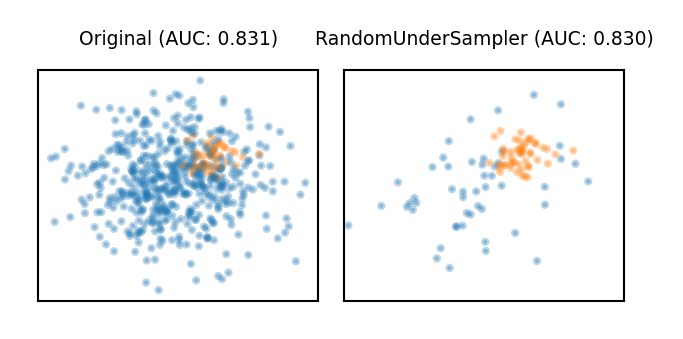
\includegraphics[width=0.75\linewidth]{images/pre-processing/random-undersampling.png}
\end{center}
\end{frame}


\begin{frame}[allowframebreaks]{Model-based Undersampling}
\begin{itemize}
    \item Edited Nearest Neighbors
    \begin{itemize}
        \item Remove all majority samples that are misclassified by kNN (mode) or that have a neighbor from the other class (all).
        \item Remove their influence on the minority samples
    \end{itemize}
    \item Condensed Nearest Neighbors
    \begin{itemize}
        \item Remove all majority samples that are \textit{not} misclassified by kNN
        \item Focus on only the hard samples
    \end{itemize}
\end{itemize}

\begin{center}
    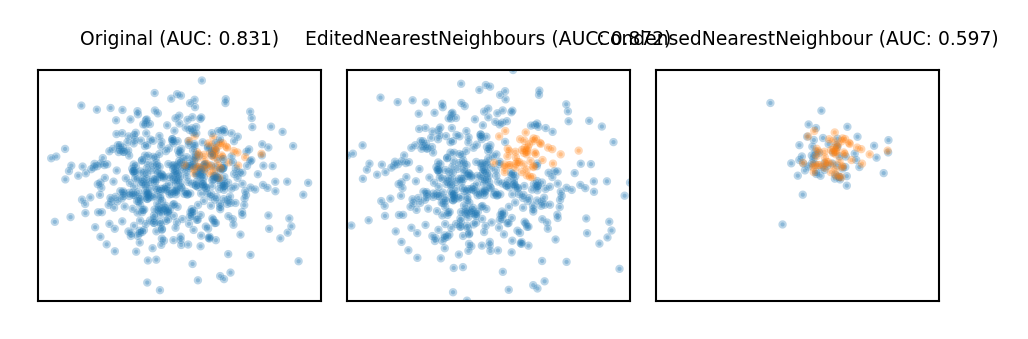
\includegraphics[width=0.75\linewidth]{images/pre-processing/model-based-undersampling.png}
\end{center}
\end{frame}


\begin{frame}[allowframebreaks]{Random Oversampling}
\begin{itemize}
    \item Copy the points from the majority class
    \item Randomly sample from the minority class, with replacement, until balanced
    \begin{itemize}
        \item Optionally, sample until a certain imbalance ratio (e.g. 1/5) is reached
    \end{itemize}
    \item Makes models more expensive to train, doesn't always improve performance
    \item Similar to giving minority class(es) a higher weight (and more expensive)
\end{itemize}

\begin{center}
    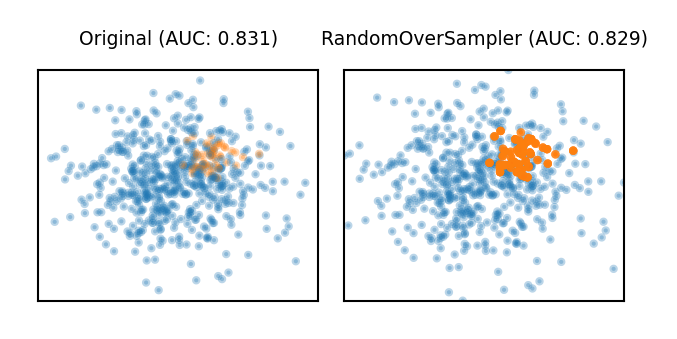
\includegraphics[width=0.75\linewidth]{images/pre-processing/random-oversampling.png}
\end{center}
\end{frame}


\begin{frame}[allowframebreaks]{Synthetic Minority Oversampling Technique (SMOTE)}
\begin{itemize}
    \item Repeatedly choose a random minority point and a neighboring minority point
    \begin{itemize}
        \item Pick a new, artificial point on the line between them (uniformly)
    \end{itemize}
    \item May bias the data. Be careful never to create artificial points in the test set.
    \item ADASYN (Adaptive Synthetic)
    \begin{itemize}
        \item Similar, but starts from 'hard' minority points (misclassified by kNN)
    \end{itemize}
\end{itemize}

\begin{center}
    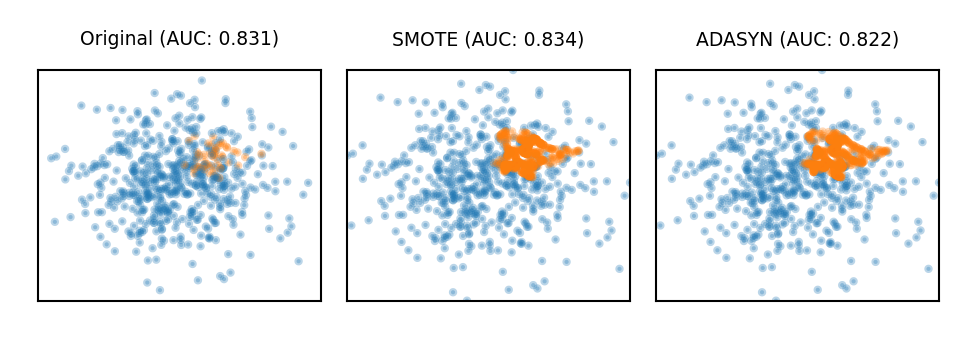
\includegraphics[width=0.85\linewidth]{images/pre-processing/smote}
\end{center}
\end{frame}


\begin{frame}[allowframebreaks]{Combined techniques}
\begin{itemize}
    \item Combines over- and under-sampling
    \item E.g. oversampling with SMOTE, undersampling with Edited Nearest Neighbors (ENN)
    \begin{itemize}
        \item SMOTE can generate 'noisy' point, close to majority class points
        \item ENN will remove up these majority points to 'clean up' the space
    \end{itemize}
\end{itemize}

\begin{center}
    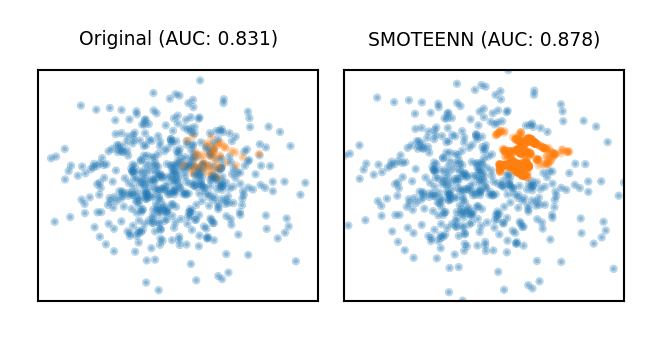
\includegraphics[width=0.85\linewidth]{images/pre-processing/smoteenn}
\end{center}
\end{frame}


\begin{frame}[fragile,allowframebreaks]{Ensemble Resampling}
\begin{itemize}
    \item Bagged ensemble of balanced base learners. Acts as a learner, not a preprocessor
    \item BalancedBagging: take bootstraps, randomly undersample each, train models (e.g. trees)
    \begin{itemize}
        \item Benefits of random undersampling without throwing out so much data
    \end{itemize}
    \item Easy Ensemble: take multiple random undersamplings directly, train models
    \begin{itemize}
        \item Traditionally uses AdaBoost as base learner, but can be replaced
    \end{itemize}
\end{itemize}

\begin{center}
    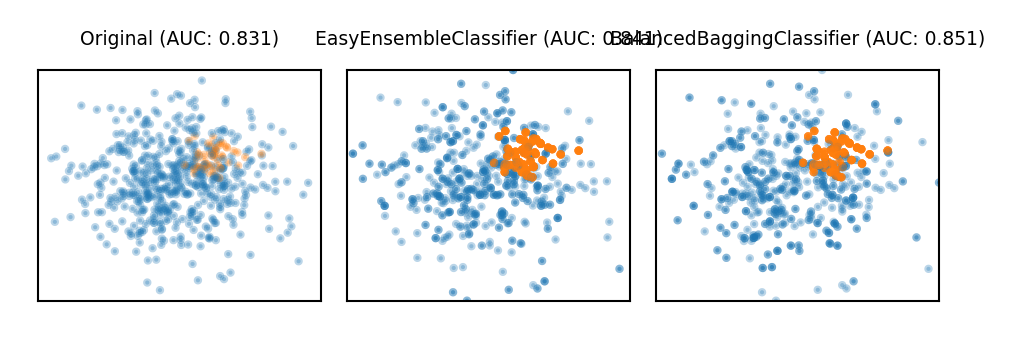
\includegraphics[width=0.9\linewidth]{images/pre-processing/ensemble-resampling}
\end{center}
\end{frame}


\begin{frame}[fragile,allowframebreaks]{Comparison}
\begin{itemize}
    \item The best method depends on the data (amount of data, imbalance,\dots)
    \begin{itemize}
        \item For a very large dataset, random undersampling may be fine
    \end{itemize}
    \item You still need to choose the appropriate learning algorithms
    \item Don't forget about class weighting and prediction thresholding
    \begin{itemize}
        \item Some combinations are useful, e.g. SMOTE + class weighting + thresholding
    \end{itemize}
\end{itemize}

\begin{center}
    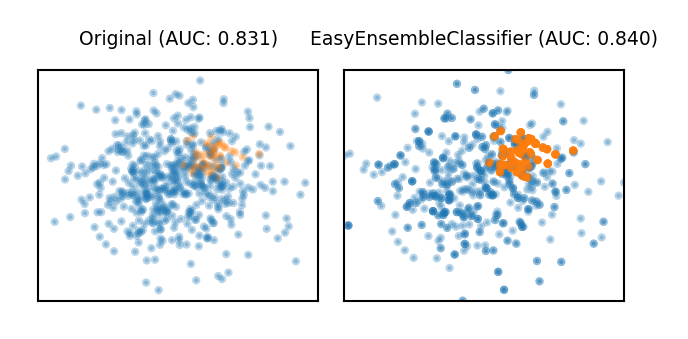
\includegraphics[width=0.9\linewidth]{images/pre-processing/sampling-compare}
\end{center}
\end{frame}


\begin{frame}[fragile,allowframebreaks]{Real-world data}
\begin{itemize}
    \item The effect of sampling procedures can be unpredictable
    \item Best method can depend on the data and FP/FN trade-offs
    \item SMOTE and ensembling techniques often work well
\end{itemize}

\begin{center}
    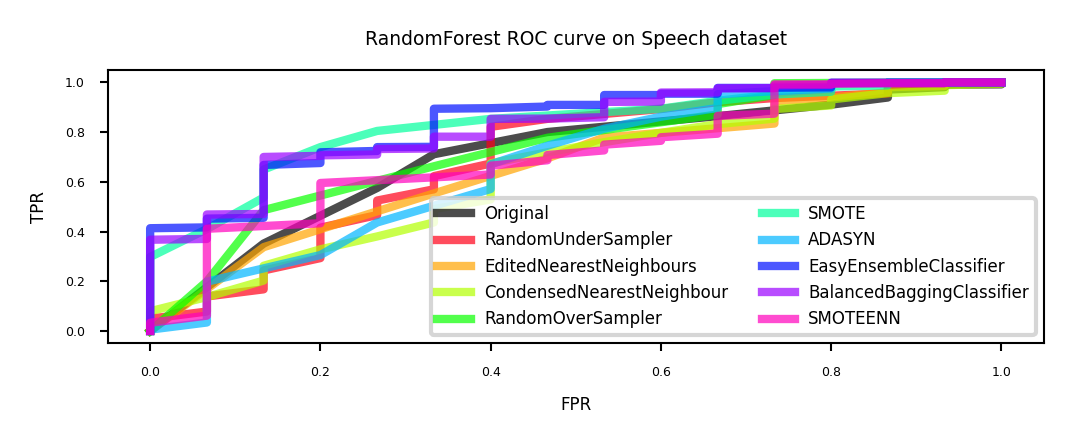
\includegraphics[width=0.95\linewidth]{images/pre-processing/sampling-effect}
\end{center}
\end{frame}
